\documentclass[conference]{IEEEtran}
% Add the compsoc option for Computer Society conferences.
%
% If IEEEtran.cls has not been installed into the LaTeX system files,
% manually specify the path to it like:
% \documentclass[conference]{../sty/IEEEtran}

\pagestyle{plain}

% *** Do not adjust lengths that control margins, column widths, etc. ***
% *** Do not use packages that alter fonts (such as pslatex).         ***
% There should be no need to do such things with IEEEtran.cls V1.6 and later.
% (Unless specifically asked to do so by the journal or conference you plan
% to submit to, of course. )


% correct bad hyphenation here
%\hyphenation{op-tical net-works semi-conduc-tor}


% Uncomment to enable anonymous submission
%\newcommand*{\ANON}{}%
% Uncomment to make the paper "submission-ready"
\newcommand*{\SUBMISSION}{}%

%  Hide URLs for anonymous submission
\ifdefined\ANON
\newcommand{\repo}{\url{https://www.dropbox.com/sh/v8ct0un8x7loi3m/AAB6op3fOWCp9qKEYlFI_Upba?dl=0}}
\newcommand{\repotamarin}{\textbf{redacted}}
\newcommand{\repoprl}{\textbf{redacted}}
\newcommand{\reposimulation}{\textbf{redacted}}
\else
\newcommand{\repo}{\url{https://github.com/EricssonResearch/v2x-self-revocation}}
\newcommand{\repotamarin}{\url{https://github.com/EricssonResearch/v2x-self-revocation/tree/main/proofs}}
\newcommand{\repoprl}{\url{https://github.com/EricssonResearch/v2x-self-revocation/tree/main/prl}}
\newcommand{\reposimulation}{\url{https://github.com/EricssonResearch/v2x-self-revocation/tree/main/simulation}}
\fi


\ifdefined\SUBMISSION
\usepackage[disable]{todonotes}
\else
\usepackage[textsize=footnotesize]{todonotes}
\presetkeys{todonotes}{fancyline}{}
\setlength{\marginparwidth}{1.3cm}
\setlength{\marginparsep}{3pt}
\fi

\newcommand{\christoph}[1]{\todo[color=orange!20]{\textbf{Christoph:} #1}}
\newcommand{\eddy}[1]{\todo[color=yellow]{\textbf{Eddy:} #1}}
\newcommand{\fritz}[1]{\todo[color=blue!20]{\textbf{Fritz:} #1}}
\newcommand{\gianluca}[1]{\todo[color=red!20]{\textbf{Gianluca:} #1}}
\newcommand{\jt}[1]{\todo{\textbf{JT:} #1}}
\newcommand{\karl}[1]{\todo[color=gray!20]{\textbf{Karl:} #1}}

\usepackage{acronym}
\usepackage{enumerate}
\usepackage{subcaption}
\usepackage{pgfplots}
\pgfplotsset{
    width=5cm, 
    legend style={
        font=\footnotesize,
        %rounded corners=2pt
    },
    compat=newest
}
\usepackage[utf8]{inputenc}
\DeclareUnicodeCharacter{2212}{−}
\usepgfplotslibrary{groupplots,dateplot}
\usetikzlibrary{patterns,shapes.arrows}
% timeline diagram
\usetikzlibrary{decorations.pathreplacing,calligraphy}

\usepackage[cmex10]{amsmath}
\usepackage{url}
\usepackage{tabularx}
\usepackage{fontawesome}

%\titleformat{\paragraph}[runin]
%{\bfseries}{\theparagraph}{1em}{}

\newtheorem{req}{Requirement}
\newtheorem{defn}{Definition}
\newtheorem{prop}{Property}

\usepackage[capitalize]{cleveref}
\crefname{figure}{Fig.\@}{Figs.\@}
\Crefname{figure}{Fig.\@}{Figs.\@}
\crefname{table}{Tab.\@}{Tabs.\@}
\Crefname{table}{Tab.\@}{Tabs.\@}
\crefname{section}{Sect.\@}{Sects.\@}
\Crefname{section}{Sect.\@}{Sects.\@}
\crefname{req}{Req.\@}{Reqs.\@}
\Crefname{req}{Req.\@}{Reqs.\@}

\usepackage{paralist}
\usepackage{crossreftools}

\usepackage{fix-cm} % not needed if not using Computer Modern

\DeclareMathAlphabet{\mathsfit}{T1}{\sfdefault}{\mddefault}{\sldefault}
\SetMathAlphabet{\mathsfit}{bold}{T1}{\sfdefault}{\bfdefault}{\sldefault}

\usepackage{listings}
\lstdefinelanguage{Tamarin}{
  keywords={lemma,All,Ex,not,rule, restriction},
  keywordstyle = {\bfseries},
  otherkeywords={&,==>,.,=,<,>},
  comment=[l]{//},
  morecomment = [s]{/*}{*/},
  morestring=*[d]{'},
  columns=fullflexible
}

\lstdefinestyle{mystyle}{
    inputpath=listings,
    commentstyle=\color{teal},
    keywordstyle=\color{magenta},
    numberstyle=\tiny\color{gray},
    stringstyle=\color{purple},
    basicstyle=\ttfamily\scriptsize,
    breakatwhitespace=false,         
    breaklines=true,                 
    captionpos=b,                    
    keepspaces=true,                 
    numbers=none,                    
    numbersep=5pt,                  
    showspaces=false,                
    showstringspaces=false,
    showtabs=false,                  
    tabsize=2
}

\lstset{style=mystyle}

\hyphenation{pseu-do-nym}
\hyphenation{pseu-do-nyms}

\newcommand{\tamarin}{\textsc{Tamarin}}
\newcommand{\tamrule}[1]{\texttt{#1}}

\newcommand{\rewire}{\textsc{Rewire}}

% TC functions
\newcommand{\funcsetup}{\textsc{Setup}}
\newcommand{\funccreate}{\textsc{Create}}
\newcommand{\funcjoin}{\textsc{Join}}
\newcommand{\funcissue}{\textsc{Create}}
\newcommand{\funcsign}{\textsc{Sign}}
\newcommand{\funcverify}{\textsc{Verify}}
\newcommand{\funcheartbeat}{\textsc{Heartbeat}}
\newcommand{\funcrevokedaa}{\textsc{Revoke}}

% names
\newcommand{\vehicle}[1]{\emph{$v_{#1}$}}
\newcommand{\tc}[1]{\emph{$\mathit{TC}_{#1}$}}
\newcommand{\ps}{\emph{$\mathit{ps}$}}

% functions and variables
\newcommand{\funcnow}{\emph{$\mathsfit{now}$}}
\newcommand{\funcgettime}{\emph{$\mathsfit{get\_time}()$}}
\newcommand{\varnow}{\emph{$\mathsfit{current}$}}
\newcommand{\funcrevoke}[1]{\emph{$\mathsfit{revoke}(#1)$}}
\newcommand{\funcrevokepar}[1]{\emph{$\mathsfit{revoke}(#1)$}}
\newcommand{\funcselfrevoke}[1]{\emph{$\mathsfit{self\_revoke}(#1)$}}
\newcommand{\funcautorevoke}{\emph{$\mathsfit{auto\_revoke()}$}}
\newcommand{\funcsignature}[1]{\emph{$\mathsfit{sig}_{\mathsf{RA}}(#1)$}}

% parameters
%\newcommand{\paramtd}{\emph{$T_{\mathsf{d}}$}}
\newcommand{\paramtd}{\emph{$\Delta$}}
\newcommand{\paramtt}{\emph{$T_{\mathsf{v}}$}}
\newcommand{\paramtr}{\emph{$T_{\mathsf{r}}$}}
\newcommand{\paramtol}{\emph{$E_{\mathsf{tol}}$}}
\newcommand{\paramed}{\emph{$T_{\mathsf{e}}$}}

% time values
% CB: some of these are times (t), others parameters for time periods (T)
\newcommand{\paramtvv}{\emph{$t_{\mathsf{v2v}}$}}
\newcommand{\paramthb}{\emph{$t_{\mathsf{hb}}$}}
\newcommand{\paramtout}{\emph{$t_{\mathsf{out}}$}}
\newcommand{\paramtrev}{\emph{$t_{\mathsf{rev}}$}}
\newcommand{\paramtsign}{\emph{$t_{\mathsf{sign}}$}}
\newcommand{\paramtrel}{\emph{$T_{\mathsf{rel}}$}}
\newcommand{\paramteff}{\emph{$T_{\mathsf{eff}}$}}
\newcommand{\paramtprl}{\emph{$T_{\mathsf{prl}}$}}
%\newcommand{\paramtra}{\emph{$t_{\mathsf{RA}}$}}
\newcommand{\paramtra}{\emph{$t$}}
\newcommand{\paramtmsg}{\emph{$t_{\mathsf{msg}}$}}

% epoch values
% CB: similar here: e = epoch identifier, E = epoch count
\newcommand{\paramera}{\emph{$e$}}
\newcommand{\paramevv}{\emph{$e_{\mathsf{v2v}}$}}
\newcommand{\paramehb}{\emph{$e_{\mathsf{hb}}$}}
\newcommand{\paramerev}{\emph{$e_{\mathsf{rev}}$}}
\newcommand{\paramesign}{\emph{$E_{\mathsf{sign}}$}}
\newcommand{\parameeff}{\emph{$E_{\mathsf{eff}}$}}
\newcommand{\parameeprl}{\emph{$E_{\mathsf{prl}}$}}
\newcommand{\paramemsg}{\emph{$e_{\mathsf{msg}}$}}

% Attackers
\newcommand{\attackerhonest}{\emph{honest}}
\newcommand{\attackersmart}{\emph{smart}}
\newcommand{\attackersmarter}{\emph{smarter}}
\newcommand{\attackerblind}{\emph{blind}}
\newcommand{\attackersmartprl}{\emph{smart-prl}}
\newcommand{\attackersmarterprl}{\emph{smarter-prl}}
\newcommand{\attackerblindprl}{\emph{blind-prl}}

% Simulation parameters
\newcommand{\simvehicles}{400}
\newcommand{\simgroups}{20}
\newcommand{\simattackers}{10\%}
\newcommand{\simrevocations}{600}
\newcommand{\simreplayrate}{30\%}
\newcommand{\simdroprate}{0.4}
\newcommand{\simdelayrate}{0.4}
\newcommand{\simcorrectrate}{20\%}
\newcommand{\simrevocationrate}{10}

% Experimental results
\newcommand{\simhonestmedian}{17}
\newcommand{\simsmartmedian}{32}
\newcommand{\simsmartmin}{24}
\newcommand{\simsmartmax}{40}
\newcommand{\simblindmedian}{20}
\newcommand{\simsmartprlmedian}{20}
\newcommand{\simsmartprlmin}{1.5}
\newcommand{\simsmartprlmax}{37.5}

\acrodef{AA}{Authorization Authority}
\acrodef{CCA}{Confidential Compute Architecture}
\acrodef{CRL}{Certificate Revocation List}
\acrodef{DAA}{Direct Anonymous Attestation}
\acrodef{ECU}{Electronic Control Unit}
\acrodef{HB}{heartbeat}
\acrodef{ITS}{Intelligent Transport System}
\acrodef{OBU}{On-Board Unit}
\acrodef{OCSP}{Online Certificate Status Protocol}
\acrodef{OSR}{Order for Self-Revocation}
\acrodef{PRL}{Pending Revocation List}
\acrodef{RA}{Revocation Authority}
\acrodef{RSU}{Road-Side Unit}
\acrodef{SCMS}{Security Credential Management System}
\acrodef{SGX}{Security Guard Extensions}
\acrodef{V2I}{Vehicle-to-Infrastructure}
\acrodef{V2P}{Vehicle-to-Pedestrian}
\acrodef{V2V}{Vehicle-to-Vehicle}
\acrodef{V2X}{Vehicle-to-Everything}
\acrodef{TC}{Trusted Component}
\acrodef{TEE}{Trusted Execution Environment}
\acrodef{TOCTOU}{Time-Of-Check-Time-Of-Use}
\acrodef{TPM}{Trusted Platform Module}

\acrodefplural{ITS}[ITS]{Intelligent Transport Systems}

\begin{document}
%
% paper title
% can use linebreaks \\ within to get better formatting as desired
\title{Demo: Efficient and Timely Revocation\\of V2X Credentials}


\ifdefined\ANON
\author{\em Anonymous Author(s)}
\else
\makeatletter
\newcommand{\linebreakand}{%
  \end{@IEEEauthorhalign}
  \hfill\mbox{}\par
  \mbox{}\hfill\begin{@IEEEauthorhalign}
}
\makeatother

\author{\IEEEauthorblockN{Gianluca Scopelliti$^{*\dagger{}}$, Christoph Baumann$^{*}$, Fritz Alder$^{\dagger{}}$, Eddy Truyen$^{\dagger{}}$, Jan Tobias M\"{u}hlberg$^{\ddagger{}\dagger{}}$}
\IEEEauthorblockA{
  \textit{$^{*}$Ericsson Security Research, Sweden;
          $^{\dagger{}}$DistriNet, KU Leuven, Belgium;
          $^{\ddagger{}}$Universit\'e Libre de Bruxelles, Belgium} \\
  \textit{gianluca.scopelliti@ericsson.com}
}
}
\fi

\IEEEoverridecommandlockouts
\makeatletter\def\@IEEEpubidpullup{6.5\baselineskip}\makeatother
\IEEEpubid{\parbox{\columnwidth}{
    Symposium on Vehicles Security and Privacy (VehicleSec) 2024 \\
    26 February 2024, San Diego, CA, USA \\
    ISBN 979-8-9894372-7-6 \\
    https://dx.doi.org/10.14722/vehiclesec.2024.25002 \\
    www.ndss-symposium.org
}
\hspace{\columnsep}\makebox[\columnwidth]{}}


% make the title area
\maketitle

\begin{abstract}
We present an interactive visual demo of our novel revocation scheme for V2X
credentials, which is the first to guarantee an upper bound on revocation time
in the presence of strong network attackers. The demo allows users to inspect
the network state with a number virtual vehicles, attackers, and events such as
network delays and service disruption.
\end{abstract}

\section{Introduction}

State-of-the-art credential management systems for \ac{V2X} proposed in industry
standards leverage \emph{pseudonymous} identities to protect the privacy of
vehicles and their passengers~\cite{brecht2018scms,etsi2022102941}. However, as
highlighted by recent
surveys~\cite{wang2020certificate,yoshizawa2022v2x_survey}, such systems present
several limitations with respect to \emph{revocation}, i.e., the capability to
punish malicious or misbehaving actors after misbehavior connected to a
participant's pseudonym is detected. To address these challenges, we have
designed a novel revocation scheme based on
self-revocation~\cite{scopelliti2024efficient}. Our scheme provides a
formally-verified design that guarantees an upper bound on revocation time and
ensures scalability even with a large numbers of vehicles and attackers in the
network. In this interactive demo, we present a proof-of-concept implementation
of our scheme applied to a simulated \ac{V2X} scenario.

\section{Scheme Overview}

In a typical \ac{V2X} scenario~\cite{brecht2018scms,etsi2022102941}, vehicles
exchange information with each other to provide functionalities such as
collision avoidance or assisted/autonomous driving. These messages are
authenticated using pseudonymous credentials (\emph{pseudonyms} in short), which
are issued by the \ac{V2X} infrastructure to vehicles upon successful
authentication and authorization, and are rotated periodically to prevent
long-term tracking of vehicles. Misbehaviour detection mechanisms are employed
to detect and report misbehaving pseudonyms, which are then \emph{revoked} to
preserve road safety.

In our revocation scheme~\cite{scopelliti2024efficient}, a \ac{RA} is
responsible for distributing periodic messages called \acp{HB}. Such messages
have a two-fold purpose: First, they carry timing information that is used by
vehicles to obtain a common notion of time, which can then provide freshness
information to network messages. Second, \acp{HB} contain a list of pseudonyms
to be revoked. Vehicles receiving a \ac{HB} first synchronize their local notion
of time with the one included in the message, and then check if any of their
pseudonyms is included in the \ac{HB}. If so, they perform
\emph{self-revocation} of their credentials. In case malicious vehicles attempt
to avert revocation, e.g., by dropping \acp{HB}, they will eventually become unable to
communicate because their local time will not advance beyond the
last \ac{HB} received. To make this scheme work, we require a \ac{TC} in each
vehicle. This \ac{TC} is responsible for the management of credentials.

\iffalse
Furthermore, to deal with network attackers that may drop or delay \acp{HB},
vehicles not receiving a \ac{HB} for a certain amount of time will eventually
get de-synchronized, effectively becoming unable to participate in future
\ac{V2X} communication. We formalized our scheme with the Tamarin
prover~\cite{meier2013tamarin}: Assuming that each network message (either
\ac{V2V} or \ac{HB}) has a validity period \paramtt{}, revocation is guaranteed
to happen within $\paramteff{}=2*\paramtt{}$ after the revocation request is
issued. Furthermore, we prove that each pseudonym added to the \ac{PRL} can be
safely removed after a time $\paramtprl{}=\paramtt{}$, guaranteeing that the
\ac{PRL} remains reasonably small.
\fi

\section{Demo Description \& Conclusions}

We have developed a proof-of-concept implementation of our scheme in a simulated
\ac{V2X} scenario running on Kubernetes. The demo consists of a number of
virtual vehicles that exchange messages with each other on a small edge area.
Attackers in the network can spread malicious information, affecting nearby
vehicles. The demo also simulates a number of real-world events such as network
delays and interruptions. The code is open source and available on
Github\footnote{https://github.com/EricssonResearch/v2x-self-revocation}.

The demo is made interactive by means of a web application where users, who play
the role of a system administrator, can monitor the state of the network and
trigger revocation requests%
%(\cref{fig:webapp})
. The application shows the state of the simulation at each time step (i.e.,
each second), and users can go back and forth in time to inspect the state of
the network. The application also shows the content of \ac{HB}
messages sent by the \ac{RA}, as well as revocation times for pseudonyms.

\iffalse
\begin{figure}
  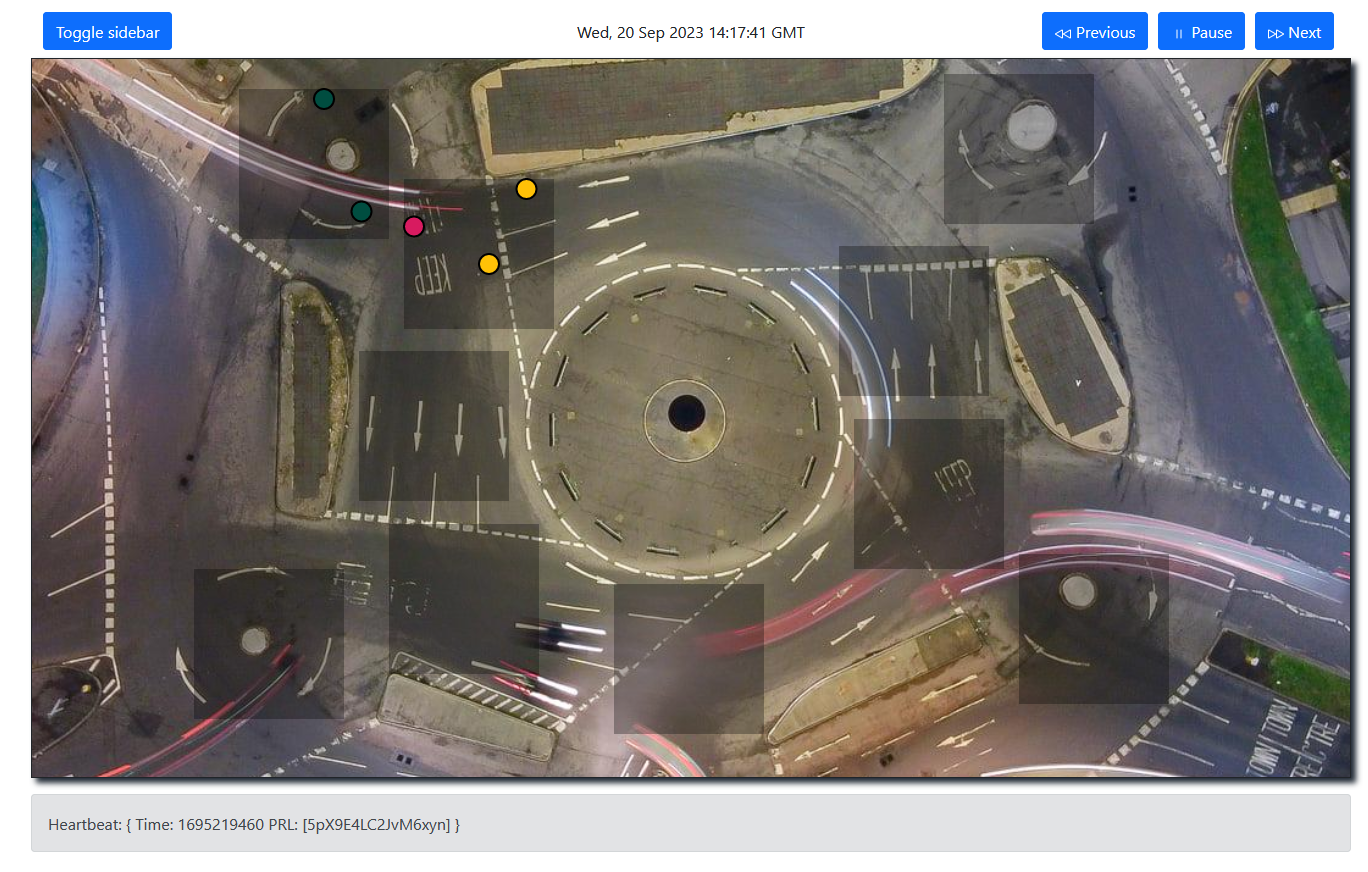
\includegraphics[width=\columnwidth]{figures/webapp.PNG}
  \caption{Screenshot of our simulation. The background shows a picture of the
  \emph{Magic Roundabout} in Swindon, UK, which is a good example of a small but
  busy edge area.}
  \label{fig:webapp}
\end{figure}
\fi

% \section{Conclusions}

This proof-of-concept demo shows the effectiveness of our revocation scheme in a
simulated but realistic \ac{V2X} scenario.

\bibliographystyle{IEEEtranS}
\bibliography{bibliography_demo}

% that's all folks
\end{document}
